\subsection{Hälsoeffekter och rekommendationer}
\subsubsection{Partiklar}
Partiklar med en diameter mindre än $10 \mu g$ (pm$_{10}$) kan komma ner och stanna i lungorna. Att utsättas för pm$_{10}$ innebär en ökad risk för att utväckla hjärt/kärlsjukdomar, andingssjukdomar samt lungcancer. Det finns ett tydligt samband mellan exponering av både pm$_{10}$ och pm$_{2,5}$ (partiklar med diameter mindre än $2,5 \mu g$) och förtida död. Det gäller också att en minskad exponering sänker dödligheten. WHO har därför satt sina rekommendarade gränsvärden för årsmedelvärde till $10 \mu g/m^3$ för pm$_{2,5}$ och till $20 \mu g/m^3$ för pm$_{10}$ \cite{whoAir}.
En svensk studie på området har kopplat samman försämrad lungfuntkion i skolåldern med utsättning för luftföroreningar från vägtrafiken i spädbarnsåldern. \cite{lungor}
\begin{figure}[H]
	\centering
	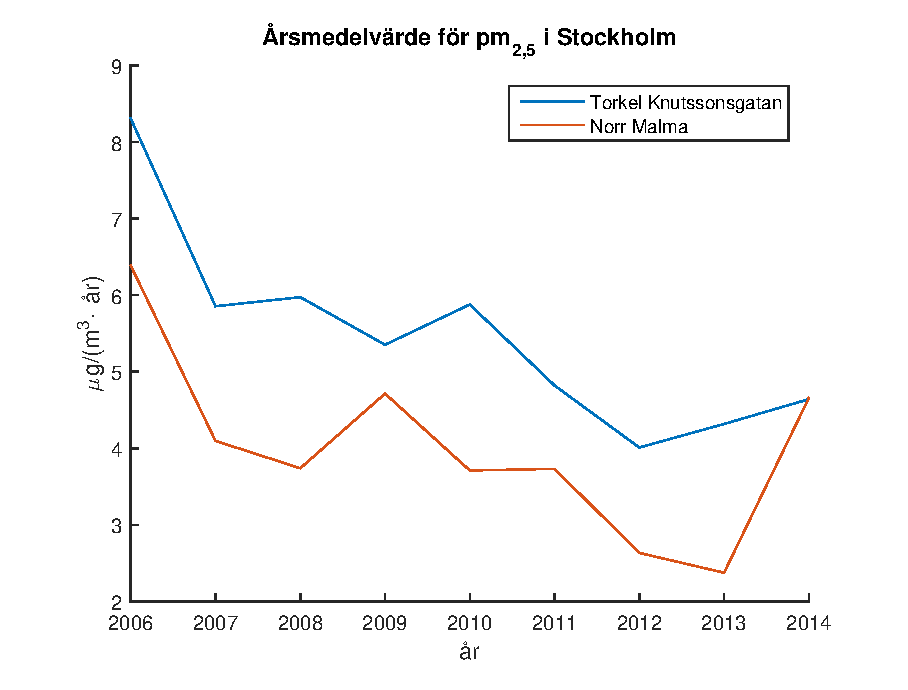
\includegraphics[width=.8\textwidth]{Bilder/pm25sth}
	\caption{Data från \url{http://slb.nu/slbanalys/historiska-data-luft/}}
	\label{fig:pm25sth}
\end{figure}

\begin{figure}[H]
	\centering
	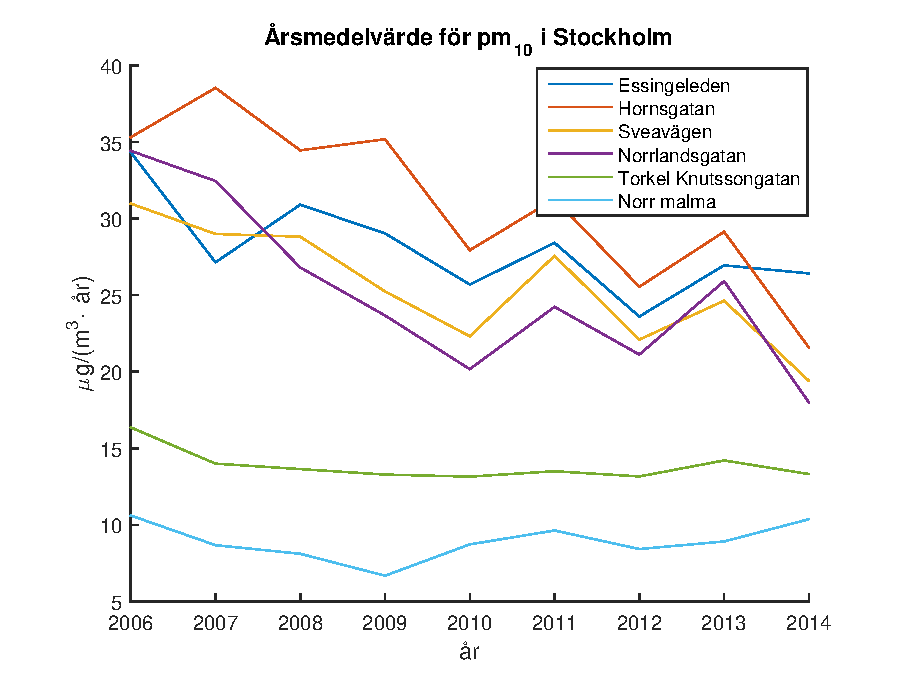
\includegraphics[width=.8\textwidth]{Bilder/pm10sth}
	\caption{Data från \url{http://slb.nu/slbanalys/historiska-data-luft/}}
	\label{fig:pm10sth}
\end{figure}

\begin{figure}[H]
	\centering
	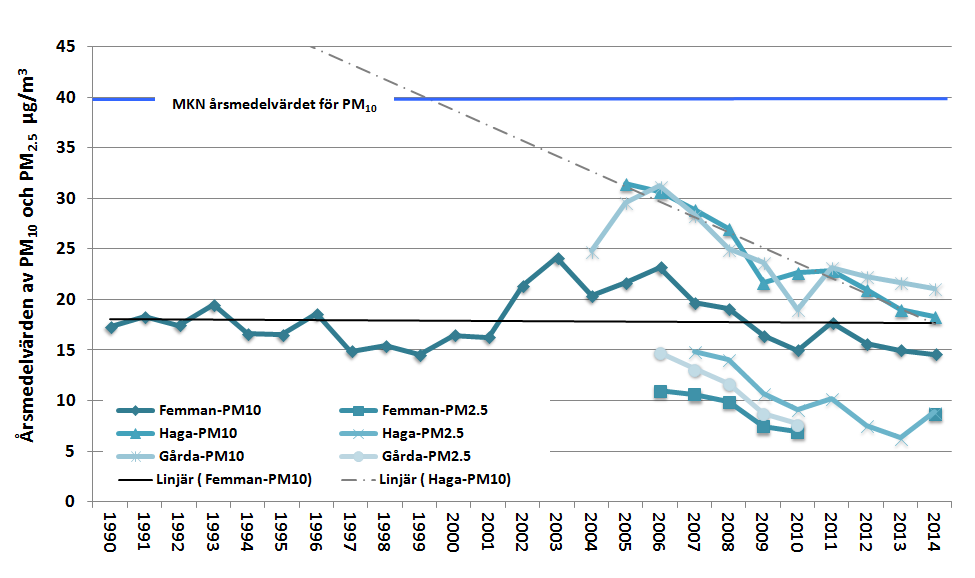
\includegraphics[width=.8\textwidth]{Bilder/pm10gbg}
	\caption{\cite{gbg}}
	\label{fig:pm10gbg}
\end{figure}
\subsection{Kvävedioxid}
Enligt \cite{whoAir} så finns det samband mellan en ökning av bronkit hos barn med astma och långvarig exponering för kvävedioxid. Samband finns också mellan minskad lungutveckling och NO$_2$ i koncentrationer som återfinns i europeiska städer idag.
\begin{figure}[H]
	\centering
	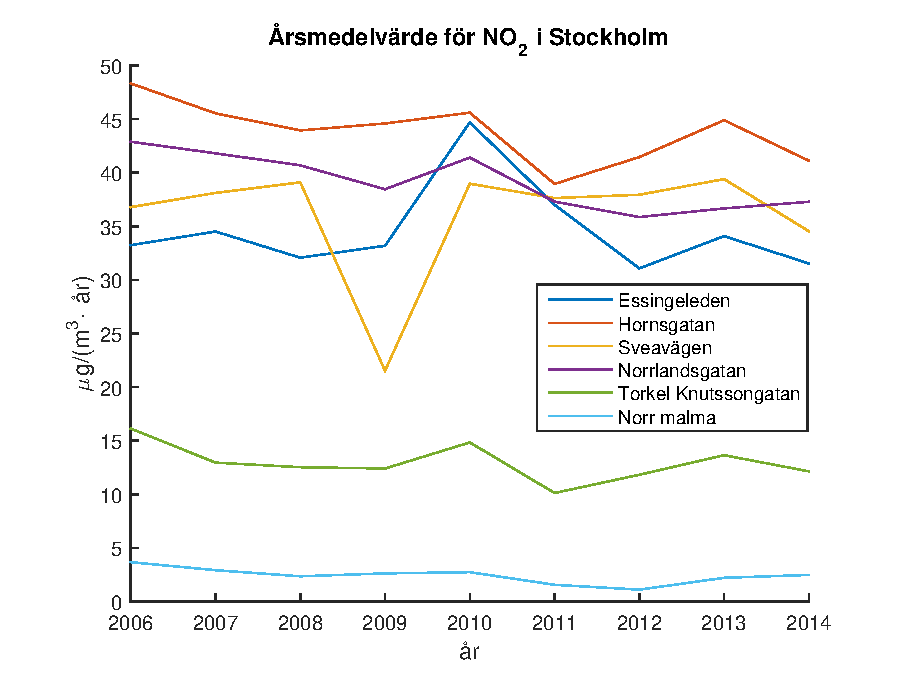
\includegraphics[width=.8\textwidth]{Bilder/NO2sth}
	\caption{Data från \url{http://slb.nu/slbanalys/historiska-data-luft/}}
	\label{fig:NO2sth}
\end{figure}

\begin{figure}[H]
	\centering
	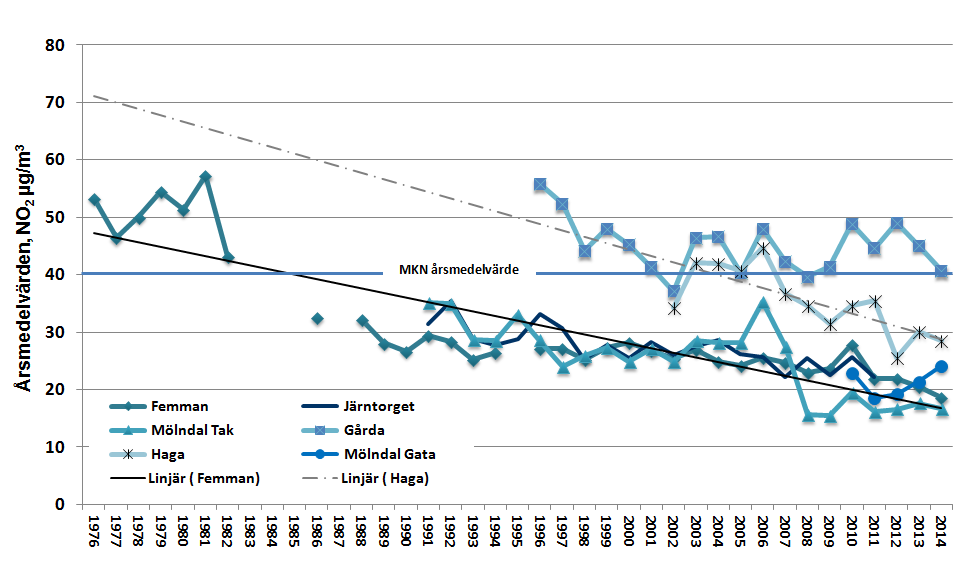
\includegraphics[width=.8\textwidth]{Bilder/NO2gbg}
	\caption{\cite{gbg}}
	\label{fig:NO2gbg}
\end{figure}
\subsection{Marknära ozon}
WHO sänkte sina riktlinjer från $120 \mu g/m^3$ till $100 \mu g/m^3$, för ett 8h glidande medelvärde, 2005. Detta för att höga halter av ozon kan ge andningsbesvär, astma, och leda till lungsjukdomar. Enligt \cite{whoAir} så leder en ökning i exponering med $10 \mu g/m^3$ till att dödligheten ökar med $0,3\%$.
\begin{figure}
	\centering
	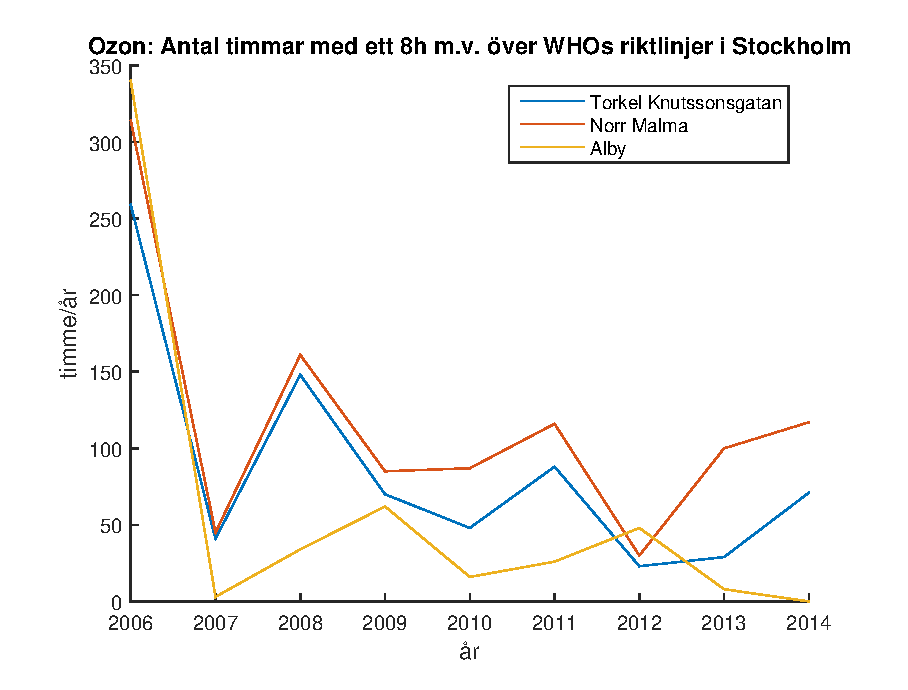
\includegraphics[width=.8\textwidth]{Bilder/ozone}
	\caption{Data från \url{http://slb.nu/slbanalys/historiska-data-luft/}}
	\label{fig:Ozone}
\end{figure}
